\documentclass{book}
\usepackage[utf8]{inputenc}
\usepackage{amsmath,amssymb,amsfonts,amsthm}
\usepackage{float}% http://ctan.org/pkg/float
\usepackage{caption}
\usepackage{algorithm}
\usepackage{algpseudocode}
\usepackage{subcaption}
\usepackage{picins}
\usepackage{mathtools}
\usepackage[calc]{adjustbox}
\usepackage{cutwin}
\usepackage{mdwlist}
\usepackage{xcolor}
\usepackage{blindtext}
\usepackage{svg}
\usepackage[english]{babel}
\usepackage{tabularx}
\usepackage{graphicx}
\usepackage{wrapfig}
\usepackage[english]{babel}
\usepackage{algorithm}
\usepackage{algpseudocode}
\usepackage{wrapfig}
\usepackage{tikz}
\usepackage{imakeidx}
\usepackage[T1]{fontenc}
\usepackage{geometry}
\definecolor{Grey1}{RGB}{84, 110, 122}
\newtheorem{Definizione}{\textbf{Definizione}}
\newcommand{\norm}[1]{\left\lVert#1\right\rVert}
\newtheorem{theorem}{Theorem}[section]
\newtheorem{corollary}{Corollary}[theorem]
\newtheorem*{Importante}{\textbf{\textcolor{red}{Importante}}}
\newtheorem{lemma}[theorem]{Lemma}
\newtheorem{esempio}{\textcolor{Grey1}{Esempio}}
\usetikzlibrary{shapes.geometric, arrows}
\geometry{a4paper, top=2cm, bottom=2cm, left=1.5cm, right=1.5cm}
\makeindex[columns=3, title=Alphabetical Index, intoc]
\title{Computer and Network Security}
\author{Lorenzo Rossi}
\graphicspath{{Images/}}
\svgpath{{Images/}}
\newlength{\strutheight}
\settoheight{\strutheight}{\strut}

\newtheorem{definition}{Definition}[section]
\newtheorem*{remark}{Remark}
\usetikzlibrary{shapes,arrows}
\tikzstyle{block} = [draw, fill=blue!20, rectangle,
    minimum height=3em, minimum width=6em]
\tikzstyle{sum} = [draw, fill=blue!20, circle, node distance=1cm]
\tikzstyle{input} = [coordinate]
\tikzstyle{output} = [coordinate]
\tikzstyle{pinstyle} = [pin edge={to-,thin,black}]
\usepackage{amsmath}
\usepackage{tikz}
\usetikzlibrary{shapes.geometric, arrows}
\usepackage{geometry}
\geometry{a4paper, top=2cm, bottom=2cm, left=1.5cm, right=1.5cm}
\usepackage{imakeidx}
\usepackage[T1]{fontenc}
\makeindex[columns=3, title=Alphabetical Index, intoc]
\title{Controllo Adattivo e Robusto}
\author{Lorenzo Rossi}
\makeindex

\graphicspath{{Images/}}
\begin{document}
\theoremstyle{definition}

\maketitle
\tableofcontents
\newpage
\section{Strumenti}
\subsection{Norma di un segnale, guadagno di un sistema}
Il controllo robusto e adattivo hanno l'obiettivo di controllare sistemi dinamici in presenza di incertezze. In particolare, il controllo robusto regola l'incertezze dinamiche mentre quello adattivo le incertezze statiche.
Le incertezze possono essere rappresentate anche come segnali esterni e quindi considerate come disturbi. Così, si da luogo alla teoria della regolazione.
\subsection{Incertezza}
I sistemi di controllo sono progettati in modo tale che certi segnali di riferimento non abbiano valori eccessivi al fine di raggiungere un valore di riferimento e mantenendo piccolo il segnale degli attuatori, responsabili del controllo. Gli attuatori sono affetti da incertezza poiché operano sul modello matematico che si basa sulle leggi fisiche che descrivono il processo.
Approssimando il sistema si introducono delle \textbf{dinamiche non modellate} che producono incertezza associate, nella maggior parte dei casi, ad alte frequenze o legate ai sensori che si utilizzano.
Queste incertezze possono essere modellate a seconda dell'obiettivo che si vuole raggiungere tramite vari metodi:
\begin{itemize}
    \item \textbf{Controllo Adattivo}: è il metodo di controllo che contiene un meccanismo di adattamento in funzione dei parametri;
    \item \textbf{Controllo Robusto}: è un metodo di controllo che garantisce le performance in presenzsa di un'incertezza limitata nel caso peggiore;
    \item\textbf{Teoria della regolazione}: l'idea è quella che i segnali esterni possano essere descritti attraverso un altro sistema dinamico al fine di garantire le performance;
    \item\textbf{Controllo stocastico} l'idea è quella che l'incertezza viene modellata tramite grandezze probabilistiche.
\end{itemize}
Di solito il problema di controllo si sviluppa in una combinazione tra le varie tecniche di controllo.

\begin{definition}[Principio di equivalenza certa]
Il \textbf{principio di equivalenza certa} dice che sostituendo ai valori veri quelli stimati, a patto che le stime abbiano proprietà di convergenza ai valori veri e favorevoli come la limitatezza e la convergenza asintotica, allora è possibile sostituire ai valori veri il corrispondente valore stimato;
\end{definition}
\begin{definition}[Principio del modello interno]
Il \textbf{principio del modello interno} duce che bisogna incorporare nel cammino del feedback un modello copiato del sistema che generato il disturbo.
\end{definition}
\begin{definition}[Metodo del gradiente]
Il \textbf{metodo del gradiente} è un metodo di ottimizzazione in cui si cerca di minimizzare il costo.
\end{definition}
\begin{definition}[Teoria della passività]
La \textbf{teoria della passività} generalizza \emph{Lyapunov} in cui si interpreta il comportamento del sistema tramite l'ingress, l'uscita e l'energia. Ci si limita allo studio dello scambio energetico di un sistema.
\end{definition}
\begin{definition}[Parametrizzazione]
La \textbf{parametrizzazione} fornisce un metodo per descrive l'incertezza di un sistema dinamico come combinazione lineare di segnali noti e quantità non note.
\end{definition}
\subsection{Norma di un segnale}
Come abbiamo detto precedentemente l'obiettivo del controllo di un sistema è quello di ottenere un comportamento desiderato e per questo motivo occorre definire il concetto di norma di un vettore.
\begin{definition}[Norma di un vettore]
Sia un vettore su spazio finito, allora definiamo la norma di un vettore come:\newline\(v\in\mathbf{R}^{n}\rightarrow\norm{v}=\sqrt{v^T v}\)
\end{definition}

Nei segnali la norma indica se il segnale è piccolo o grande e come è facilmente intuibile dipende dal tipo di norma utilizzata. Questo perché un segnale può apparire più o meno grande in base alla norma scelta.
Quindi, assumiamo che un segnale \(r(t):\mathbf{R}\rightarrow\mathbf{R}^n\), allora è possibile definire le seguenti norme.
\begin{definition}[Norma 2]
All'istante t: \(r^t(t)t(t) \geq 0\)
Integrando in tutto il dominio del segnale e normalizzando il segnale:
\begin{center}
    \(\sqrt{\int_{0}^{\infty}r^T(\tau)r(\tau)d\tau}\)
\end{center}
\end{definition}
Tuttavia, non è detto che questo integrale converga.
\begin{definition}[Segnale limitato]
Il segnale \(r(t)\in\mathbf{R}^2\( è limitato se \)\norm{r}_2\) è limitato. 
\end{definition}
\begin{remark}
\begin{itemize}
    \item convergenza asintotica \(\rightarrow r(t)\rightarrow0\\t\rightarrow\infty\)
    \item Non fornisce nessua informazione sulla limitatezza del segnale.
\end{itemize}
\end{remark}
\begin{definition}[Norma 1]
Dato un segnale \(r(t)\int\mathbf{R}_n\) si definisce la norma 1 del segnale:
\begin{center}
    \(\norm{r}_1=\int_{0}^{\infty} |r_1(t)+|r_2(t)|+..d\tau=\sum_{i=1}^{n}|r_{i}(t)d\tau\)
\end{center}
\end{definition}
\begin{remark}
\begin{itemize}
    \item sengale che converge a zero più veloce della norma 2.
    \item Non fornice informazione sulla limitatezza del segnale.
\end{itemize}
\end{remark}
\begin{definition}[Norma \(\infty\)]
Dato un segnale \(r(t)\int\mathbf{R}_n\) si definisce la norma infinito:
\begin{center}
    \(\norm{r}_{\infty}=\max_{i=1}^{n} sup|r_i(\tau)|\)
\end{center}
\end{definition}ù
\begin{remark}
\begin{itemize}
    \item La norma infinito da informazioni sulla limitatezza del segnale poiché:
    \begin{itemize}
        \item si considera il masismo assoluto;
        \item si considera il massimo assoluto da tutte le componenti;
    \end{itemize}
    Quindi tutte le componenti del segnale sono al di sotto del masismo.
\end{itemize}
\end{remark}
\begin{definition}[Norma p]
Dato un segnale \(r(t)\int\mathbf{R}_n\) si definisce la norma p:
\begin{center}
    \(\norm{r}_p=(\int_{0}^{\infty}|r(\tau)|^pd\tau)^{1/p}=(\int_{0}^{\infty}\sum_{i=1}^{n}|r_i(\tau)|^p d\tau)^{1/p}\)
\end{center}
\end{definition}
\begin{remark}
\begin{itemize}
    \item Fornisce proprietà di convergenza;
    \item Non fornisce informazioni sulla limitatezza del segnale.
\end{itemize}
\end{remark}
Per analizzare la \textbf{stabilità} si deve utilizzare la norma 1 o la norma 2 e per le proprietà di convergenza e limitatezza la norma infinito.
\begin{definition}[Segnale di potenza]
Dato un segnale \(r(t):\mathbf{R}:\rightarrow\mathbf{R}^n\) è un \textbf{segnale di potenza} se;
\begin{center}
    \(pow(r)=lim_{T\rightarrow \infty} \frac{1}{T}\int_{0}^{T}r(t)^2 \partial \tau\) è finito.
\end{center}
\end{definition}
\begin{remark}
\begin{itemize}
    \item Se \(\norm{r}_2\(è limitata \)\rightarrow pow(r) =0\);
    \item Se \(\norm{r}_\infty\( è definito \)\rightarrow pow(r)\leq \norm{r}_\infty\) e si possono avere segnali illimitati.
\end{itemize}
\end{remark}
\begin{definition}[Norma indotta]
Considerato un vettore \(v\in \mathbf{R}^n\( tale che \)w=Av\in\mathbf{R}^p\) definiamo la \textbf{norma indotta} della matrice \(A\):
\begin{center}
    \(\norm{A}_{indotta}=\sup_v\frac{\norm{w}_2}{\norm{v}_2}=\sup_v\frac{\sqrt{v^TA^TAv}}{\sqrt{v^Tv}}\) se finita.
\end{center}
\end{definition}
Estendendo questo concetto ai sistemi si può considerare la seguente situazione:
\begin{center}
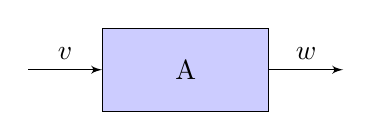
\begin{tikzpicture}[auto, node distance=2cm,>=latex']
    % We start by placing the blocks
    \node [input, name=input] {};
    \node [block, right of=input](A){A};
    \node [output, right of=A] (output) {};
    
    \draw [->] (input) -- node{\(v\)} (A);
    \draw [->] (A) -- node{\(w\)} (output);
\end{tikzpicture}
\end{center}
In cui \(w\( è una amplificazione di \)v\).
\subsection{Guadagno di un sistema}
\begin{definition}[\textbf{Guadagno di un sistema}]
Il \textbf{guadagno di un sistema} è la misura di amplificazione considerando ingressi \(u\in\mathbf{R}^p\( e uscite \)y\in\mathbf{R}^p\) con il suo massimo.
\begin{center}
   \begin{tikzpicture}[auto, node distance=2cm,>=latex']
    % We start by placing the blocks
    \node [input, name=input] {};
    \node [block, right of=input](?){?};
    \node [output, right of=?] (output) {};
    
    \draw [->] (input) -- node{\(\norm{u}_p\)} (A);
    \draw [->] (A) -- node{\(\norm{y}_p\)} (output);
    \end{tikzpicture} 
\end{center}
\end{definition}
\begin{remark}
Se le norme sono limitate, allora il guadagno è limitato.
\end{remark}
  Nei sistemi lineari è possibile utilizzare norme diverse per ingressi come l'impulso di Dirac. Le relative proprietà del sistema vengono rappresentate nel dominio della frequenza come per esempio il \textbf{margine di fase e/o di guadagno}.
  Queste proprietà caratterizzano la \textbf{robustezza} del sistema.
  \begin{theorem}
    La norma \(L_2\( di un sistema SISO lineare, tempo invariante, asintoticamente stabile coincide con la distanza in \)\mathbb{C}\) tra l'origine e il punto più lontano nel diagramma di Nyquist.
  \end{theorem}
  \begin{remark}
  In un sistema dinamico:
  \begin{center}
  \begin{equation}
      \begin{cases}
        \dot{x}=Ax+Bu\\
        y=Cx+Du
      \end{cases}
  \end{equation}
      \end{center}
definiamo la matrice di traferimento nel dominio delle frequenze \(G(jw)\), il massimo valore della risposta in freqeunza, se il sistema è asintoticamente stabile, vale:
\begin{center}
    \(\norm{G}_\infty=\sup_w|G(jw)|=\norm{G}_{2_{indotta}}\)
\end{center}
  \end{remark}
\textbf{Esercizio}\newline
\begin{equation}
    G(s)=\frac{as+1}{bs+1}\quad a\geq0,b>0
\end{equation}
Dato che \(a\geq0\rightarrow\( assenza di zeri a fase non minima inolte \)b>0\rightarrow\) il sistema è asintoticamente stabile.
\begin{remark}
Nei sisrwmi lineari propri, l'esistenza di una norma implica l'esistenza delle altre norme e viceversa, legandosi così alla proprietà di asintotica stabilità. Tuttavia, questo non è vero nei sistemi non lineari.
\end{remark}
\subsection{Lemma di Barbalat}
\subsubsection{Stabilità di Lyapunov}
\begin{definition}[Stabilità secondo Lyapunov]
Considerato un sistema dinamico con lo stato \(x\( e un punto di equilibrio \(x_e\( e con \(x_0\) lo stato in \)t=0\). Il punto di equilibrio è \textbf{stabile secondo Lyapunov} se:\newline \)\exists \varepsilon>0,\exists\delta=\delta(\varepsilon)>0\) tale che:
\begin{center}
    \begin{equation}
        \norm{x_0-x_e}<\delta\rightarrow\norm{x(t)-x_e}<\varepsilon \forall t\geq 0
    \end{equation}
\end{center}
\end{definition}
La \(\varepsilon\( è legata alle prestazioni future del sistema con \)\delta\) il vincolo sulle condizioni iniziali che garantiscono la limitatezza negli istanti futuri.\newline
\textbf{Esericzio}
\begin{equation}
    \begin{cases}
      \dot{x_1}=\psi(t,x_1,x_2)x_2\\
      \dot{x_2}=-\psi(t,x_1,x_2)x_1
    \end{cases}, \psi(t,x_1,x_2)>0 \quad \forall t,x_1,x_2
\end{equation}
Dimostra che il sistema ha un unico punto di equilibrio nell'origine.
\begin{equation}
    \begin{bmatrix}
    \dot{x_1}\\\dot{x_2}
    \end{bmatrix}=
    \begin{bmatrix}
    0 & \psi\\-\psi&0
    \end{bmatrix}
    \begin{bmatrix}
    x_1\\x_2
    \end{bmatrix}
\end{equation}
\begin{equation}
    x_1\dot{x_1}+x_2\dot{x_2}=0\rightarrow\frac{\partial (\frac{x_1^2}{2}+\frac{x_2^2}{2})}{\partial t}=0
\end{equation}
Se è costante in \(t\):
\begin{equation}
    \frac{x_1^2}{2}+\frac{x_2^2}{2}=\frac{x_1(0)^2}{2}+\frac{x_2(0)^2}{2}
\end{equation}
Quindi, scelto un \(\varepsilon\( fissiamo \)\delta(\varepsilon)\) tale che l'evoluzione futura del sistema sia limitato. In questo caso è stabile, ma non asintoticamente stabile poiché non converge a 0. Come si può evedere in figura:
\begin{center}
    \includesvg[scale=1.3]{Lyapunov.svg}
\end{center}

\begin{definition}[Punto attrattivo]
Un punto di equilibrio \(x_e\) si dice \textbf{attrattivo} se tutte le traiettorie con le condizioni iniziali convergono al punto di equilibrio.
\end{definition}
\begin{remark}
La proprietà di attrattività è diversa dalla proprietà di stabilità.
\end{remark}

\begin{definition}[Stabilità asintotica]
Un punto di equilibrio \(x_e\) è \textbf{stabile asintoticamente} se è stabile attrattivo.
\end{definition}
\begin{theorem}[Teorema di stabilità di Lyapunov]
  Consideriao un sistema autono non lineare descritto da:
  \begin{equation}
      \dot{x} = f(x) \quad x(t)\in X\in \mathbb{R}^n
  \end{equation}
  Assumiamo \(x_e=0\( punto di equilibrio tale che \)f(0)=0,x(t)=0  \forall t\geq0\) ed inoltre:\begin{itemize}
      \item autovalori di \(\frac{\partial f(0)}{\partial x}\) siano nella parte sinistra del piano complesso;(\textbf{Criterio di Linearizzazione})
      \item esiste una matrice definita positiva \(V:x\rightarrow\mathbb{R}^{\geq 0}\ (t.c V(0)=0, \ V(x)>0 \ \forall x \neq 0)\( tale che \)V_xf(x)<0 \ \forall x\neq 0\) in un intorno del'origine. (\textbf{Principio di Lasalle})
  \end{itemize}
  Allora il punto di equilibrio \(x_e\) è localmente asintoticamente stabile
\end{theorem}
\begin{remark}
\item \textbf{Linearizzazione}\\
    \begin{equation}
        \dot{x}=f(x)
    \end{equation}
    \begin{equation}
        \dot{x}=Ax+o(\norm{x}^2)
    \end{equation}
    In cui la matrice \(A=\frac{\partial f(0)}{\partial x}\). Quindi, se:
    \begin{equation}
        \forall \lambda_i\in\sigma(A)\geq0\in\mathbb{C} \rightarrow Asintoticamente\ stabile\ in\ un\ intorno\ di\ x_e
    \end{equation}
    Inoltre, se \(Re(\lambda)<0\ \forall \lambda_i \), l'andamento è esponenziale.\newline
\textbf{Principio di Lasalle}
Se
\begin{equation}
    \exists V:x\rightarrow\mathbb{R}^{\geq0}
\end{equation} funzione di Lyapunov, allora rappresenza l'energia del sistema tale che:
\begin{equation}
    \begin{cases}
      V(0)=0\quad in\ x_e\\V(x)>0\quad\forall x\neq 0
    \end{cases}
\end{equation} con \(V_xf(x)<0\quad\forall x\neq 0\) in un intorno dell'origine.
\end{remark}
\textbf{Applicazione Teaorema Lyapunov}\newline
\begin{center}
    \includesvg[scale=1]{appLyap.svg}
\end{center}
 \(V(x)>0 \rightarrow insieme chiuso e limitato\)\newline
Per valutare la funzione di Lyapunov occorre valutare il suo gradiente in un punto:\newline
\(V_{x}^{T}f<0\quad x\neq 0\rightarrow\dot{x}\in\(al settorer interno della linea di livello da \)t\rightarrow t+\partial t\rightarrow \dot{x}\) viene attratta verso l'interno.
Tramite Lyapunov, inoltre, è possibile valutare le condizioni di stabilità:
\begin{center}
    \emph{Se prende una condizione iniziale nella circonferenza di raggio \(\delta\varepsilon\(, questa potrebbe uscire dala circonferenza dei raggio \(\delta\varepsilon\), ma deve rimanere all'interno della circonferenza di raggio \)\varepsilon\) (più grande) per poi convergere a zero}
\end{center}
\begin{remark}
Se gli insieme di livello della funzione di Lyapunov sono limitati allora \(\exists\forall\varepsilon>0\) t.c. le condizioni di Lyapiunov sono soddisfatte.
\end{remark}
\begin{remark}
Per avere l'asintotica stabilità, inegrando lo Jacobiano della funzione di Lyapunov, le traiettorie tendono ad insiemi di livello sempre più piccole e si fermano in \(V(x)=0\) in cui si ha un solo punto
\end{remark}
Quindi, la teoria di lyapunov è utile per capire le proprietà di \textbf{stabilità} e \textbf{attrattività} nel punto di equiliubrio. Tuttavia, lo svantaggio è che occorre trovare la corretta funzione di Lyapunov e il sistema deve essere autonomo, cioè senza ingresso/uscita/disturbo.
\subsubsection{Teorema di Barbalat}
  Il teorema dei Barbalat viene utilizzato nei sistemi SISO per determinare la convergenza dei segnali senza utilizzare una funzione di Lyapunov.
  \begin{definition}[Lemma di barbalat]
  Supponiamo un segnale \(r(t)=\begin{bmatrix}
  r_1(t)\\...\\r_n(t)
  \end{bmatrix}\in L_\infty\cap L_2 \( e \(\dot{r}\in L_\infty \). Allora: 
  \(lim_{t\rightarrow\infty} r(t)=0\)
  \end{definition}
  \begin{remark}
  \begin{itemize}
      \item \(L_\infty\cap L_2 \) implica un segnale infinito;
      \item \(\dot{r(t)}\in L_\infty\) è necessario per la convergenza;
      \item \textbf{Lemma di Barbalat debole}:
      \(r\in L_\infty\( non è necessario ma \(r\in L_2 e \dot{r}\in L_\infty\) Allora: \)lim_{t\rightarrow\infty} r(t)=0\);
      \item si può utilizzare anche la norma p;
      \item \(\dot{r}\in L_\infty\) è necessario.
  \end{itemize}
  \end{remark}
  Il lemma di Barbalat può essere un'alternativa al principio di invarianza di Lasalle, ma richiede l'invarianza nel tempo.
  \textbf{ESERCIZI: pag, 14-15 degli appunti.}
  \subsubsection{Metodo del Gradiente}
  \begin{definition}[Gradiente di \(f\)]
   Consideriamo il problema di minimizzar euna funzione \(f:\mathbb{R}^{n}\rightarrow R\).\newline
  Questa è una funzione continua e derivabile e definiamo il gradiente di \(f\):
  \begin{center}
      $\nabla f=\begin{bmatrix}
      \frac{\partial f}{\partial x_1}\\ \vdots\\ \frac{\partial f}{\partial x_n}
      \end{bmatrix}$
  \end{center}
  \end{definition}
 Se \(\nabla f(x)=0\rightarrow\) \textbf{punti stazionari}(massimo, minimo, flesso)
 \begin{lemma}
 Consideriamo una funzione \(f\) continuamente differenziabile e la dinamica del sistema è costituita da:
 \begin{center}
     \(\dot{x}=-\nabla f(x)\)
 \end{center}
 Quindi, tutte le traiettorie del sistema convergono in un punto stazionario della funzione \(f\). Inolte:
 \begin{itemize}
     \item Se \(f\) è radialmente illmitata allora tutte le traiettorie sono limitate;
     \item Se \(f\( è convessa allora tutte le traiettorie convergono in un insieme minimizzatore globare di \)f\)
 \end{itemize}
 \end{lemma}
 \textbf{Esercizio}(Vedere pagina 16)\newline
 Supponiamo \(f\( quadratica: \(f(x)=\frac{1}{2}x^T Q x+c^T x+d\quad Q=Q^T\( e assumi che \(Q\succ 0\) definita positiva e \)f\) convessa. Mostra che il sistema \)\dot{x}=-(Qx+c)\) ha un unico punto di equilibrio asintoticamente stabile.
 \subsection{Dissipatività}
 La teoria della dissipatività permette lo studio delle proprietà dei sistemi interconnessi usando una prospettiva basata su considerazioni energetiche.\newline
 Consideriamo un sistema non lineare \(\Sigma\) descritto da:
 \begin{center}
 \begin{equation*}
          \dot{x}=f(x.u)\quad y=h(X,U)
 \end{equation*}
 \begin{equation*}
     x(t)\in X\subset\mathbb{R}^n;\quad u(t)\in U\subset\mathbb{R}m;\quad y(t)\in Y\subset \mathbb{R}^p;\quad f,h\  vettoriali\ e\ differenziabili
 \end{equation*}
 \end{center}
 \begin{definition}[Supply rate]
  Nello spazio \(U\times Y\) delle variabili esterne (ingresso e uscita), definiamo la funzione \textbf{supply rate} come:
  \begin{center}
      \begin{equation*}
          s:U\times Y\rightarrow \mathbb{R}
      \end{equation*}
      \includesvg[scale=0.7]{supply}
  \end{center}
 \end{definition}
 
 \begin{definition}[Sistema dissipativo]
  Un sistema \(\Sigma\( è detto \textbf{dissipativo} rispetto alla supply rate \(S\) se \)\exists S:X\rightarrow R^{\geq 0}\), detta \textbf{funzione di storage}, tale che;
  \begin{center}
      \begin{equation*}
          \forall t_1\geq t_0,\quad\forall u\quad \quad S(x(t_1))\leq S(x(t_0))+\int_{t_0}^{t_1} S(u(\tau),y(\tau))\partial\tau
      \end{equation*}
  \end{center}
  In cui lo stato \(x(t_1)\( deve essere limitato superiormente dalla funzione di storage e l'integrale della supply rate. Inoltre, se l'equazione viene soddisfatta con il segno di uguaglianza \(\forall x(t_0),t_1\geq t_0\( e tutti gli \(u_{[t_0,t_1]}\) allora \)\Sigma\) è detta \textbf{loseless} rispetto a \)\Sigma\), cioè che non vi è dissipatività.
 \end{definition}
 \begin{remark}
 La \textbf{disuguaglianza dissipazionale} ci dice che l'energia immagazzinata nel sistema in \(t_1\( è al massimo uguale all'energia immagazzinata nell'istante iniziale \)t=0\) e a tutte l'energia immagazzinata dall'esterno. Quindi non vi è \textbf{creazione di energia}
 \end{remark}
 La disuguaglianza dissipazionale è:\begin{center}
      \begin{equation*}
          \forall t_1\geq t_0,\quad\forall u\quad \quad S(x(t_1))\leq S(x(t_0))+\int_{t_0}^{t_1} S(u(\tau),y(\tau))\partial\tau
      \end{equation*}
 \end{center} 
 Essa dipende dalle traiettorie del sistema, ma quello che vogliamo fare è slegare questa dipendenza. Quindi:
 \begin{center}
     \begin{equation*}
         S(x(t))-S(x(t_0))\leq\int_{t_0}^{t} S(u,y)\partial\tau\quad t\geq rt_0
     \end{equation*}
     \begin{equation*}
         \frac{ S(x(t))-S(x(t_0))}{t-t_0}\leq\frac{\int_{t_0}^{t} S(u,y)\partial\tau}{t-t_0}
     \end{equation*}
     \begin{equation*}
         lim_{t\rightarrow t_0}\frac{ S(x(t))-S(x(t_0))}{t-t_0}\leq lim_{t\rightarrow t_0}\frac{\int_{t_0}^{t} S(u,y)\partial\tau}{t-t_0}
     \end{equation*}
     \begin{remark}
     Questo è possibile poiché \(S\) è differenziabile.
     \end{remark}
     Applicando la differenziabilità per la parte sinistra della disequazione e il teorema di De Hopital per il membro destro, si ottiene:
     \begin{equation*}
         S_{x}f(x,0)\leq S(u,y)\leq S(u,h(x,u))
     \end{equation*}
     Se \(u=0\):
     \begin{equation*}
         S_{x}f(x,0)\leq S(0,h(x,0))=0
     \end{equation*}
 \end{center}
\subsection{Passività}
una scelta particolare di supply rate, tipica del controllo adattativo) è:\begin{center}
    \begin{equation*}
    s(u,y)=u^Ty
\end{equation*}
\end{center}
Questo è possibile se e solo se il numero di input è uguale a quello di output e quindi il sistema viene detto \textbf{quadrato}.\newline
Supponiamo \(\Sigma\( dissipativo rispetto alla supplyrate appena definita. Allora per qualche funzione \(S\geq0\( e \)\forall x(0),T\geq0\) e tutti i segnali di input \)u_{[0,T]}\):
\begin{center}
    \begin{equation*}
        S(x(t))\leq S(x(0))+\int_{0}^{T} u^T(\tau)y(\tau)\partial\tau
    \end{equation*}
    \begin{equation*}
        \int_{0}^{T} u^T(\tau)y(\tau)\partial\tau\geq  S(x(t))- S(x(0))\geq -S(x(0))
    \end{equation*}
\end{center}
Quindi, la massima energia estratta dal sistema è limitata superiormente e dipende dalla funzione di storage iniziale.
\begin{definition}[Sistema Passivo]
 Dato un sistema \(\Sigma\), esso è:
 \begin{itemize}
     \item \textbf{passivo} se risulta dissipativo rispetto alla supply rate \begin{equation*}
    s(u,y)=u^Ty
\end{equation*};
\item \textbf{strettamente passivo rispetto all'ingresso} se è possibile determinare:
    \begin{equation*}
        \exists \delta>0 t.c sistema dissipativo con S(u,y)=u^Ty-\delta\norm{u}^2
    \end{equation*}
\item \textbf{stettamente passivo rispetto all'uscita} se:\begin{equation*}
    \exists \varepsilon t.c sistema dissipativo con S(u,y)=u^Ty-\varepsilon\norm{y}^2
\end{equation*};
\item \textbf{conservativo} se è loseless rispetto a  \begin{equation*}
    s(u,y)=u^Ty
\end{equation*}
 \end{itemize}
\end{definition}
\begin{remark}
I termini con il segno meno nella passività rispetto all'ingresso e all'uscita rappresentano termini di sconto per la supply rate.
\end{remark}
\subsection{Condizioni di Hill-Moylan e KYP} 
L'obiettivo delle \textbf{condizioni di Hill-Moylan e KYP} è quello di disaccoppiare le condizioni sugli stati e gli ingressi rispetto alla dissipatività. A tale scopo consideriamo sistemi \textbf{affini nelle variabili di ingresso} (lineari).
\begin{definition}[Classe di Sistema]
 Definiamo la \textbf{classe di sistemi} \(\Sigma_a\) tutti quesi sistemi descritti da:\begin{equation*}
     \dot{x}=f(x)+g(x)u\quad y=h(x)
 \end{equation*}
\end{definition}
\begin{theorem}[Teorema Hill e Moylan]
  Considerato il sistema affine \(\Sigma_a\), supponiamo, inoltre, che il sistema sia passivo con una funzione differenziabile di sotrage S. Allora:\begin{equation*}
      S_xf(x)\leq0\quad S_xg(x)=h^T(x)
  \end{equation*}
\end{theorem}
\begin{proof}
Se \(f(x,u)\leq S(u,h(x,u))\rightarrow\) \begin{equation*}
    S_x[f(x)+g(x)u]\leq u^Ty=h^T(x)u
\end{equation*}
Se \(u=0\):\begin{equation*}
    S_xf\leq0
\end{equation*}
Fissato \(x\( e \)u\in\mathbb{R}\):\begin{equation*}
    \begin{bmatrix}\vdots\\
    S_xf\\
    \vdots
    \end{bmatrix}
    +
    \begin{bmatrix}\vdots\\
    S_xg-h^T\\ \vdots
    \end{bmatrix}u\leq0
\end{equation*}
che rappresenta l'equazione di una retta:
\begin{center}
    \includesvg{DimHILL.svg}
\end{center}
Appena aumenta si va oltre \(z=0\) e la disuguaglianza risulta non verificata;\begin{equation*}
    \alpha=0\rightarrow S_xg-h^T=0
\end{equation*}
Quindi:
\begin{equation*}
    S_xg(x)=h^T(x)
\end{equation*}
\end{proof}
\begin{remark}
\begin{itemize}
    \item Le condizioni di Hill-Moylan generalizzano il teorema di Lyapunov, poiché se il sistema è asintoticamente stabile secondo Lyapunov, allora:\begin{equation*}
        S:xf(x)\leq0
    \end{equation*}
    risulta soddisfatta.
    \item Sono condizioni più restrittive dato che:\begin{equation*}
        S_xg(x)=h^T(x)
    \end{equation*}
    \item Permette l'interconnessione tra sistemi dato che si considerano più ingressi e uscite.
\end{itemize}
\end{remark}
Supponiamo \(\Sigma\):
\begin{equation*}
    \dot{x}=f(x)+g(x)u
\end{equation*}
Il punto \(x=0\( è \textbf{stabile} se \(\exists V\succ0\) tale che \)V_xf\geq0\)\newline
Vogliamo chiderci se esiste un \(y\( tale che \)\Sigma\) sia passiva. Questo è possibile definendo:\begin{equation*}
    y=h(x)\quad h(x)=g^TVx^T
\end{equation*}
\begin{equation*}
    \Sigma: \begin{cases}
      \dot{x}=f(x)+g(x)u\\y=g^T(x)Vx^T
    \end{cases} \ un \ sistema \ passivo.
\end{equation*}

\begin{theorem}[KYP]
  Consideriamo la classe di sistemi \(\Sigma_a\). Supponiamo il sistema lineare:\begin{equation*}
      \dot{x}=Ax+Bu\\y=Cx
  \end{equation*}
  e che \(\Sigma\) sia passiavo con una funzione di storage quadratica:\begin{equation*}
      S(x)=\frac{1}{2}x^TPx\quad P=P^T\succ 0
  \end{equation*}
  Allora:\begin{equation*}
      A^TP+PA\leq0\quad PB=C^T
  \end{equation*}
\end{theorem}
\begin{remark}
\begin{equation*}
      \dot{x}=Ax+Bu\quad y=Cx
  \end{equation*}
  \begin{equation*}
      x^TPAx+x^TA^TPx\leq0
  \end{equation*}
  \begin{equation*}
      x^TPB=x^TC^T\rightarrow PB = C^T
  \end{equation*}
  Rappresenta \textbf{l'uscita passiva del sistema}. Quindi:\begin{center}
      \textbf{\(\forall P \exists!\) uscita passiva.}
  \end{center}
\end{remark}
\begin{theorem}[]
  Consideriamo la classe di sistemi \(\Sigma_a\). Supponiamo che il sistema sia strettamente passivo rispetto all'uscita con una funzione differenziale di storage S. Allora:\begin{equation*}
      S_xf(x)\leq-\varepsilon h^T(x)h(x)\quad S_xg(x)=h^T(x)
  \end{equation*}
\end{theorem}
\begin{proof}
\begin{equation*}
    S_x(f+gu)\leq y^Tu-\varepsilon h^Th
\end{equation*}
\begin{itemize}
    \item \(u=0\rightarrow\)\begin{equation*}
        S_xf\leq -\varepsilon h^T h\leq0
    \end{equation*}
    è una condizione più stringente a causa di un margine di negatività
    \item \(u\neq0\(, è verificare se è presente un termine lineare e quindi \)S_xg=h^T(x)\)
\end{itemize}
\end{proof}
\textbf{ESERCIZIO}
\begin{center}
    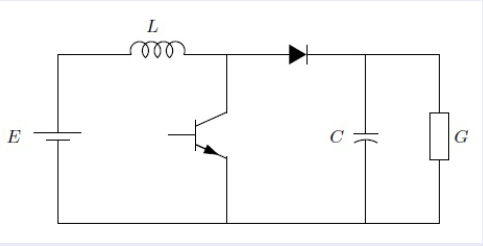
\includegraphics[scale=0.5]{DC-DCboost.png}
\end{center}
Consideriamo un boost DC-DC descritto dalle seguenti equazioni:
\begin{center}
    \begin{equation*}
        \begin{cases}
          L\dot{x_1}=-s x_2+E\quad (uscita)\\
        C\dot{x_2}=s x_1-G x_2 \\
        y=x_1
        \end{cases}\quad L>0\quad C>0\quad G>0\quad E>0\ ingresso\quad s\in\{0,1\} segnale\ di\ switching
    \end{equation*}
\end{center}
Dimostra che il sistema è passivo con funzione di storage:\begin{equation*}
    S(x_1,x_2)=\frac{L}{2}x_1^2+\frac{C}{2}x_2^2
\end{equation*}
\textbf{\emph{Svolgimento}}
Occorre verificare le condizioni di Moylan:\begin{equation*}
    \begin{cases}
      S_xf\leq0\\S_xg=0
    \end{cases}
\end{equation*}
\begin{equation*}
    S_x=\begin{bmatrix}
    Lx_1 & Cx_2
    \end{bmatrix}\quad
    f=\begin{bmatrix}
    -\frac{s}{L}x_2\\
    s\frac{x_1}{C}-\frac{G}{C}x_2
    \end{bmatrix}\quad
    g=
    \begin{bmatrix}
    \frac{1}{L}\\0
    \end{bmatrix}\quad h=x_1
\end{equation*}
\begin{enumerate}
    \item \begin{equation*}
        S_xg=\begin{bmatrix}
    Lx_1 & Cx_2
    \end{bmatrix}\begin{bmatrix}
    \frac{1}{L}\\0
    \end{bmatrix}=x_1=h
    \end{equation*}
    \item \begin{equation*}
        S_xf=\begin{bmatrix}
    Lx_1 & Cx_2
    \end{bmatrix}\begin{bmatrix}
    -\frac{s}{L}x_2\\
    s\frac{x_1}{C}-\frac{G}{C}x_2
    \end{bmatrix}=\begin{bmatrix}
    -sx_1x_2\\sx_1x_2-Gx_2^2
    \end{bmatrix}=-Gx_2^2\leq0
    \end{equation*}
    \begin{remark}
    \begin{itemize}
        \item \(sx_1x_2\) rappresenta l'energie scambiata e dato che si trovano su entrambe le righe è possibile semplificare
        \item \(-Gx_2^2\) rappreenta il termine dissipazionale.
    \end{itemize}
    \end{remark}
\end{enumerate}
L'unione di \(1+2\) implica che il sistema è passivo con quella funzione di storage che rappresenta l'energia totale del sistema.
\begin{remark}
Non si può concludere che il sistema è passivo strettamente all'uscita poiché l'uscita è \(x_1\(, ma la negatività viene data da \)x_2\). Quindi vi sono 2 uscite. In particolare:
\begin{center}
    \includesvg[scale=1.2]{EsercizioPowerPassivit}
\end{center}
\end{remark}
\subsection{Positive realness-Reale positivtà}
Consideriamo un sistema lineare:
\begin{equation*}
    \dot{x}=Ax+Bu\quad y=Cx \quad S(u,y)=u^Ty=y^Tu
\end{equation*}
Associamo a questo sistema una funzioe di trasferimento:
\begin{equation*}
    G(s)=C[sI-A]^-1B\quad G(jw)=C(jwI-A)^-1B
\end{equation*}
Inoltre, assumiamo che il sistema sia raggiungibile e osservabile ed in particolare il numero di ingressi è pari al numero delle uscite e che il sistema sia minimo. Allora sono equivalenti:
\begin{itemize}
    \item Il sistema è passivo con funzione quadratico di storage \(S(x)=\frac{1}{2}x^TPx\quad P=P^T\succ0\);
    \item Esiste la matrice \(P=P^T\succ0\( e \)L\) tale che:\begin{equation*}
        \begin{cases}
          A^TP+PA=-L^TL\\PB=C^T
        \end{cases}\quad\textbf{Teorema di KYP}
    \end{equation*}
    \item tutti i poli di \(G(S)\) siano tutti a parte reale non positiva:\begin{enumerate}
        \item Siccome \(\Sigma\) minimo allora i poli del sistema coincidono con gli autovalori della matrice A
        \item La \(A\( risolve la disuguaglianza di Lyapunov \)A^TP+PA\leq0\)
    \end{enumerate} Da queste due condizioni tutti i pli sono nella parte chiude del piano complesso
    \item \begin{enumerate}
        \item \(\forall \omega\( tale che \(j\omega\) non è polo di \)G(s)\rightarrow G(j\omega)+G^T(-j\omega)\succeq0\) semidefinita positiva
        \item \(\forall \omega\( tale che \(j\omega\) è un polo semplice \)\rightarrow Res(j\omega)=lim_{s\rightarrow j\omega}(s-j\omega)G(s)\succeq0\) è semidefinita positiva e Hermitiana
    \end{enumerate}
\end{itemize}
\begin{definition}[Funzione reale positiva]
Una funzione di trasferimento \(G(s)\) è detta \textbf{reale positiva} se soddisfa:\item \begin{enumerate}
        \item \(\forall \omega\( tale che \(j\omega\) non è polo di \)G(s)\rightarrow G(\omega)+G^T(-j\omega)\succeq0\) semidefinita positiva
        \item \(\forall \omega\( tale che \(jw\) è un polo semplice \)\rightarrow Res(j\omega)=lim_{s\rightarrow \omega}(s-\omega)G(s)\succeq0\) è semidefinita positiva e Hermitiana
    \end{enumerate}
\end{definition}
\begin{definition}[Strettamente reale positiva]
Una funzione di trasferimento \(G(s)\( è detta \textbf{strettamente reale positiva} se \(G(s-\varepsilon)\) è una funzione positiva reale per quale \)\varepsilon>0\).
\end{definition}
Per i sistemi SISO, lineari, raggiungibili e osservabili vale la proprietà:\begin{equation*}
    G(jw)+G(-jw)=2Re[G(jw)]
\end{equation*}
poiché è definita positiva se si applica la definizione di reale positiva. Quindi la proprietà di passivita ci diche che \(2Re[G(j\omega)]\geq0\) che corrisponde alla condizione di stabilità nel diagramma di Nyquist: il diagramma di Nyquist della funzione di trasferimento giace nella parte destra del piano complesso.
\begin{remark}
Ciò è possibile solo se il grado relativo della funzione di trasferimento non è ne zero ne uno.
\end{remark}
\begin{remark}
\begin{itemize}
    \item Indipendentemente dall aproprietà del sistema, la funzione di traaferimento appartiene alla parte destra del diagramam di Nyquist;
    \item Se \(D=0\rightarrow\( il grado relativo, cioè la differenza tra poli e zero è \)\geq1\). Inoltre, questa condizione viene violata ad alte frequenze.
\end{itemize}
\end{remark}
\begin{remark}
Un sistema passivo o una funzione di trasferimento reale positivo ha grado relativo nullo o 1.
\end{remark}
\begin{lemma}[C.N.S strettamente reale positivo]
Un sistema lineare, raggiungibile e osservabile SISO è \textbf{strettamente reale positivo} se e solo se tutti i poli di \(G(s)\( hanno parte reale negativa; \(Re[G(j\omega)]>0\ \forall \omega\in[0,\infty)\) e \)G(\infty)>0\ o\ lim_{\omega\rightarrow\infty}\omega^2Re[G(i\omega)]>0\)
\end{lemma}
\textbf{ESERCIZI}
\emph{Dimostra che le funzionid i trasferimento sono reali positive}
\begin{enumerate}
    \item \(G(s)=\frac{1}{s}\rightarrow G(j\omega)=\frac{1}{j\omega}=-\frac{j}{\omega}\)
    \begin{center}
    \includesvg[scale=1]{1sujomega.svg}
\end{center}
\(G(s)\( reale positva, ma non strettamente\)\mathbb{\rightarrow} Re(G(jw))=0\)
Poiché \(G(s)\) non è strettamente positiva:\begin{equation*}
    G(s-\varepsilon)=\frac{1}{s-\varepsilon}\quad\varepsilon>0
\end{equation*}
Deve essere soddisfatta l'equazione di Lyapunov con \(P=P^T\succ0\quad A^TP+PA=-L^TL\ PB=C^T\)\newline
Poiché \(\lambda A=\varepsilon\geq0\rightarrow \sigma(A)\subset\mathbb{C}^+\), il sisterma nonè passivo e quindi non reale positivo.
\item \(G(s)=\frac{1}{s^2+s+1}\), il sistema non è passivo, quindi non è reale positivo poiché il grado relativo è pari a 2.\begin{center}
    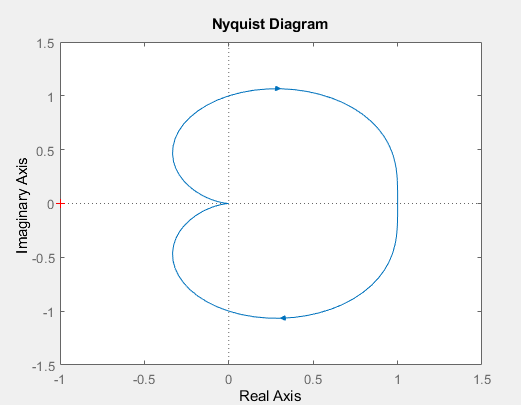
\includegraphics[scale=0.5]{1sus2s1.png}
\end{center}
\item \(G(s)=\frac{1}{s+a}\quad a>0\) \begin{equation*}
    deg(G(s))=1\rightarrow sistema stabile
\end{equation*}
Quindi valutiamo la parte reale della funzione di trasferimento e nyquist.\begin{itemize}
    \item Da Nyquist: \(|\angle G(j\omega)|\leq\frac{\pi}{2}\quad \forall\omega\in[0,\infty]\)
    \begin{center}
        \includesvg[]{1susa}
    \end{center}
    Come si può notare vi è uno sfasamento di \(\frac{\pi}{2}\(. Ora occorre valutare la funzione di trasferimento:\(Re[G(j\omega)]>0\ \forall \omega\in[0,\infty)\) e \)G(\infty)>0\ o\ lim_{\omega\rightarrow\infty}\omega^2Re[G(i\omega)]>0\).\newline
    Non valutiamo \(G(\infty)>0\) poiché il grado relativo è pari ad 1. Quindi:\begin{equation*}
        G(s-\varepsilon)=\frac{1}{s-\varepsilon+a}=\frac{1}{\Tilde{a}}\quad 0<\varepsilon\leq a,a>0
    \end{equation*}
    Allora, posso sempre trovare un \(\varepsilon\( ed in particolare, se \(\varepsilon=a\) \)G(s-\varepsilon)\) è reale positiva, ma non strettamente e quindi la funzione di trasferimento è strettamente reale positiva.
    \item \(G(s)=\frac{s}{s^2+\Tilde{\omega}^2}\quad\omega\neq0\)
    Se \(\omega=0\) si ha una cancellazione polo-zero con una conseguente perdita di raggiungibilità e osservabilità.\begin{center}
        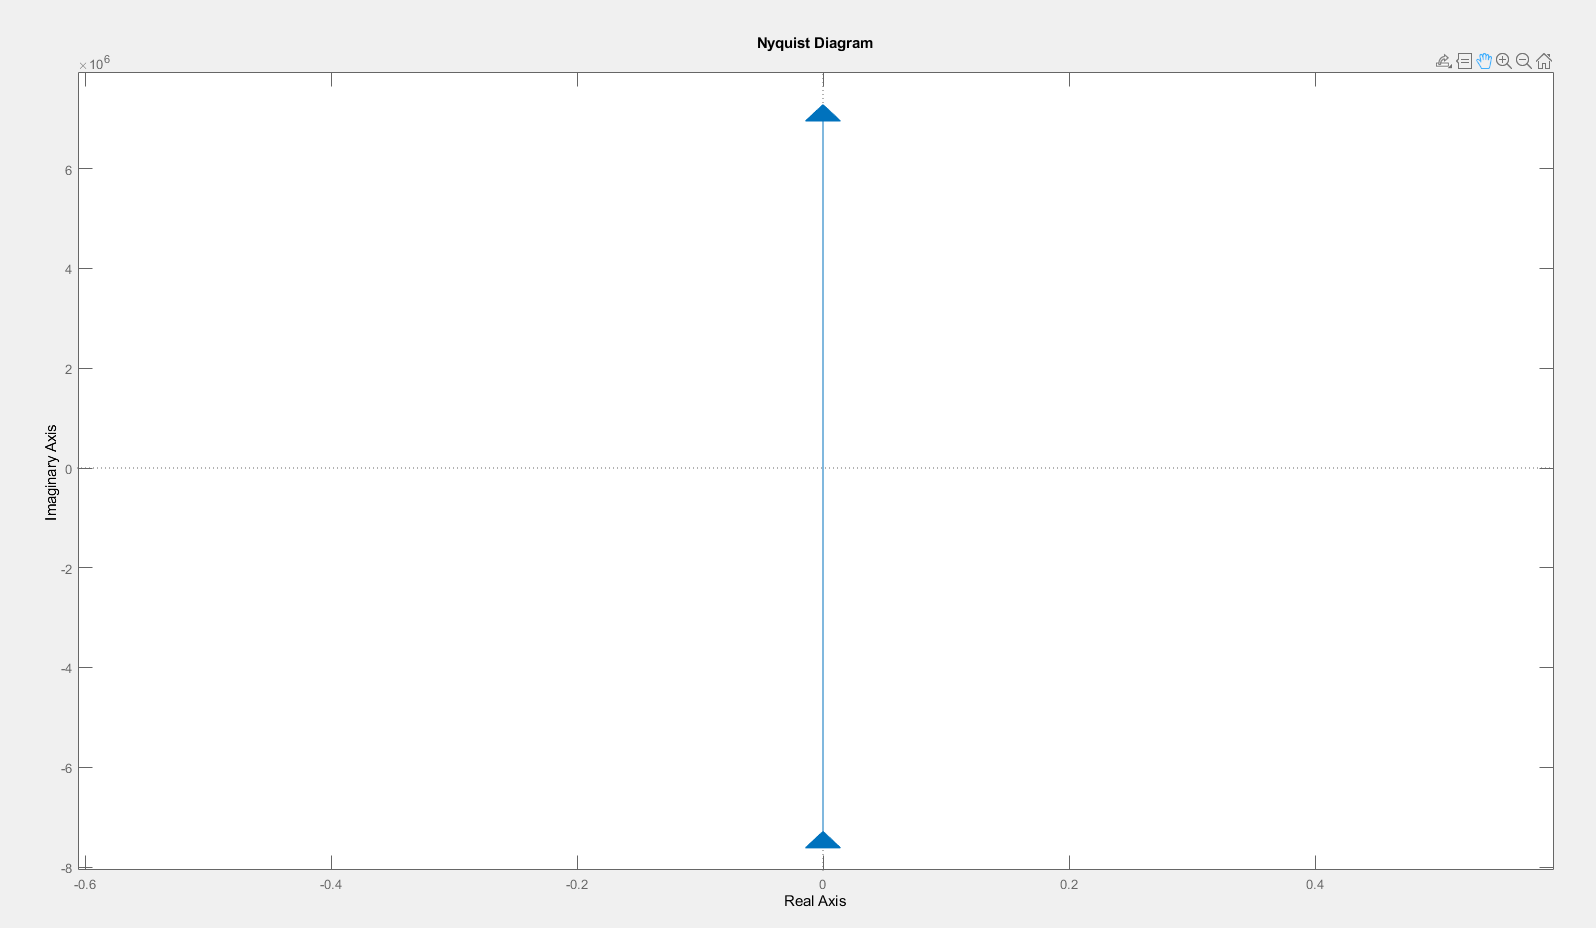
\includegraphics[scale=0.2]{susomega.png}
    \end{center} Ora:\begin{equation*}
        G(j\omega)=\frac{j\omega}{\Tilde{\omega}^2-\omega^2}
    \end{equation*}
    Il suo grado relativo è pari ad 1 ed è stabile dato che: \(\lambda(A)={j\Tilde{\omega},-j\Tilde{\omega}}\) 2 poli sull'asse immaginario.
    \begin{equation*}
        \angle G(j\omega)=\pm \frac{\pi}{2}\quad al\ variare\ di\ \omega
    \end{equation*}
    \(\forall |G(j\omega)|=\frac{\pi}{2}\( funzione di trasferimento reale positiva non strettamente e per dimostrarlo si ricorre a \)G(j\omega)+G(-j\omega)=0\)
\end{itemize}
\end{enumerate}
\subsection{Guadagno \(L_2\)(Controllo robusto)}
Definito \(\gamma\geq0\) il guadagno del sistema, consideriamo la supply rate:\begin{equation*}
    S(u,y)=\frac{1}{2}(\gamma^2\norm{u}^2-\norm{y}^2)
\end{equation*}
Supponiamo che il sistema \(\Sigma\( sia dissipativo rispetto alla supply rate. Allora per qualche funzione \)S\geq0\ \forall x(0),\ u\in[0,T]\) vale:\begin{equation*}
    \frac{1}{2}\int_{0}^{T}(\gamma^2\norm{u}^2-\norm{y}^2)\partial\tau\geq S(x(T))-S(x(0))
\end{equation*}
Quindi:\begin{equation*}
    \int_{0}^{T}\norm{y}^2\leq\gamma^2\int_{0}^{T}\norm{u}^2+2S(x(0))
\end{equation*}
cioè che il sistema \(\Sigma\( ha un guadagno \)L_2\leq\gamma\).\newline
Si dice anche che il sistema è affetto da \textbf{bias}.
\begin{definition}[Guadagno \(L_2\)]
Il sistema \(\Sigma\( possiede un guadagno \(L_2\) minore o pari a \)\gamma\) se è dissipativo rispetto alla supply rate:\begin{equation*}
    S(u,y)=\frac{1}{2}(\gamma^2\norm{u}^2-\norm{y}^2)
\end{equation*}
\end{definition}
\begin{theorem}
  Consideriamo la classe di sistemi \(\Sigma_a\(. Supponiamo che il sistema abbia guadagno \(L_2\leq\gamma>0\) con un funzione differenziale di storage \)S\). Allora:\begin{equation*}
      S_x(f(x)+g(x)u)\leq\frac{1}{2}(\gamma^2\norm{u}^2-\norm{y}^2)
  \end{equation*}
\end{theorem}
\begin{proof}
Se \(u=0\):\begin{equation*}
    S_xf+\frac{\norm{h}^2}{2}\leq 0
\end{equation*}
Se \(u\neq0\), occorre trovare la u del teorema tale che:\begin{equation*}
     S_x(f(x)+g(x)u)-\frac{1}{2}\gamma^2\norm{u}^2+\frac{1}{2}\norm{h}^2\leq0
\end{equation*}
Per \(x\( fissato è una parabola concava e per verificare che sia soddisfatta \)\forall u\) occorre trovare il punto di massimo effettuando la derivata prima. Si ottiene:\begin{equation*}
    U^{*}=\frac{1}{\gamma^2}g^T(x)S_x^T
\end{equation*}
Che, sostituita nella disuguaglianza, si giunge all'\textbf{equazione di Hamilton-Jacobi} nelle derivare parziali della funzione di storage:\begin{equation*}
    S_xf(x)+\frac{1}{2}S_xg(x)g^T(x)S_x^T+\frac{1}{2}h^T(x)h(x)\leq 0
\end{equation*}
\end{proof}
\begin{theorem}
  Consideriamo il sistema lineare:\begin{equation*}
      \begin{cases}
        \dot{x}=Ax+Bu\\y=Cx
      \end{cases}
  \end{equation*}
  osservabile. Allora sono equivalenti:\begin{enumerate}
      \item Il sistema ha guadagno \(L_2<\gamma\( con \)\gamma>0\)
      \item Esiste definita positiva \(P=P^T\) tale che:\begin{equation*}
          A^TP+PA+P\frac{BB^T}{\gamma^2}P+C^T\leq 0
      \end{equation*}
      \item Tutti gli autovalori hanno parte reale negativa ed esiste la matrice Hamiltoniana:\begin{equation*}
          H=\begin{bmatrix}
          A & \frac{BB^T}{\gamma^2}\\-C^TC & -A^T
          \end{bmatrix}\in\mathbb{R}^{2n\times2n}
      \end{equation*}
      che non abbia autovalori sull'asse immaginario.
      \item Esiste la matrice \(X=X^T\succ0\) che risolve la disuguaglianza lineare matriciale:\begin{equation*}
          \begin{bmatrix}
          A^TX+XA & XB & C^T\\ B^TX & -\gamma I & 0\\C & 0 & -\gamma I
          \end{bmatrix}<0
      \end{equation*}
  \end{enumerate}
\end{theorem}
\begin{proof}
\(\textbf{1}\Leftrightarrow\textbf{2}\): banale poiché il sistema è quadrato e basta applicare la definizione.\newline
\(\textbf{2}\Leftrightarrow\textbf{4}:\) Si dimostra tramite il complemento di Shur.\newline
\(\textbf{3}\Leftrightarrow\textbf{1}:\)
\begin{equation*}
    H=\begin{bmatrix}
    A & \frac{BB^T}{\gamma^2}\\-C^TC & -A^T
    \end{bmatrix}\quad
    J=\begin{bmatrix}
    0& I\\-I & 0
    \end{bmatrix}
\end{equation*}
\begin{equation*}
    J^-1HJ=\begin{bmatrix}
    0& -I\\I & 0
    \end{bmatrix}\begin{bmatrix}
    A & \frac{BB^T}{\gamma^2}\\-C^TC & -A^T
    \end{bmatrix}\begin{bmatrix}
    0& I\\-I & 0
    \end{bmatrix}=-H^T
\end{equation*}
\begin{equation*}
    \lambda(H)=\lambda(-H^T)=\lambda(-H)
\end{equation*}
Ricordiamo la proprietà dell'Hamiltoniano:\begin{enumerate}
    \item Autovalori simmetrici;
    \item Autovalori simmetrici rispetto all'asse immaginario;
    \item Per autovalori sull'asse immaginario non si avrà una coppia.
\end{enumerate}
Quindi \(J^-1HJ\( è simile a \(-H^T\( e \(\lambda\) simile a \)-\lambda\in\sigma(A)\) se e solo se l'autovalore non si trova sull'asse immaginario. Riscrivendo \)H\):\begin{equation*}
    H=L+MN=\begin{bmatrix}
    A & 0 \\ -C^TC & -A^T
    \end{bmatrix}+\begin{bmatrix}
    \frac{B}{\gamma}\\0
    \end{bmatrix}\begin{bmatrix}
    0 & \frac{B^T}{\gamma}
    \end{bmatrix}
\end{equation*}
\(L\) non ha autovalori sull'asse immaginario.
Supponiamo per assurdo che \(\exists \lambda=j\omega\) allora essite un autovettore destro per H:\begin{equation*}
    (L+MN)v=j\omega V\rightarrow MNv=(j\omega I-L)v\footnote{\((j\omega I-L)v\)  Non singolare}
\end{equation*}
\begin{equation}
    (j\omega I-L^-1)MNv=v\longrightarrow w=Nv\rightarrow \omega=N(j\omega I-L)^{-1}Mv
\end{equation}
Ora supponiamo che \(G(s)=C(sI-A)^-1B\):\begin{equation*}
    N(j\omega I-L)^{-1}=\frac{G(-j\omega)^TG(j\omega)}{\gamma^2}
\end{equation*}
\begin{equation*}
    \omega^T\frac{G(-j\omega)^TG(j\omega)}{\gamma^2}\omega=\omega^TN(j\omega-L)^{-1}\omega\Leftrightarrow \norm{\omega}^2=\frac{\norm{G(j\omega)\omega}^2}{\gamma^2}
\end{equation*}
Quidni:\begin{equation*}
    \norm{G(j\omega)}=\gamma
\end{equation*}
Applicando \(u=sin(\omega t)\(, la \(y\( sinusoidale con ampiega \(\gamma\( volte di \)u\). Quindi un sistema ha un guadagno \)L_2\) di valore \)\gamma\) il che rappresenza una contraddizione.
\end{proof}
\begin{remark}
Per un sistema SISO lineare, allora:\begin{itemize}
    \item La \textbf{passività} coincidere con \(G(s)\( reale positiva, allora il diagramma di nyquist giace a destra del piano e il modulo della fase è compreso tra \)[0,\frac{\pi}{2}]\);
    \item La \textbf{passività} implica la stabilità del sistema e quindi a fase minima di grado relativo pari ad 1;
    \item Il \textbf{guadagno \(L_2\(} deve essere minor di \(\gamma\). Se ciò è verificato si ha asintotica stabilità e da Nyquist tutte le traiettorie di w sono racchiuse in una circonfeenza di raggio \)\gamma\);
    \item \(G(s)\( è strettamente passiva e quindi \(G(s)=\frac{G(s)-1}{G(s)+1}\) ha un guadagno \)L_2<1\)
\end{itemize}
\end{remark}
\subsection{Stabilità e stabilizzazione di sistemi dissipativi}
\subsubsection{Stabilità di sistemi dissipativo}
\begin{theorem}
  Cinsideriamo il sistema \(\Sigma\). Supponiamo:\begin{itemize}
      \item \(\Sigma\( dissipativo con funzione differenziale di storage \)S\);
      \item \(\Sigma\( con punto di equilibrio \(x\( per \)u=0\) e \)h(x,0)=0\);
      \item \(x\) è minimizzatore stetto locale di S;
      \item La supply rate è tale che \(S(0,y)<0\quad \forall y\neq0\)
  \end{itemize}
  Allora \(x\( è un punto di equilibrio stabile per il sistema \(\dot{x}=f(x,0)\(. In aggiunta, l'unica soluzione di \(\dot{x}=f(x,0)\) tale che \)y(t)=0\quad\forall t\) è \)\dot{x}=x\). Allora, il punto di equilibrio del sistema è asintoticamente stabile.
\end{theorem}
\begin{proof}
\begin{equation*}
    S_xf\leq S(u,y)\xrightarrow[]{u=0} S_xf(x,0)\leq S(0,y)<0\quad y\neq0\quad y=h(x,0)\quad (Attorno\ al\ punto\ di equilibrio)
\end{equation*}
\begin{equation*}
    \dot{S}=S_xf(x,0)\leq S(0,y)<0
\end{equation*}
\end{proof}
\begin{definition}[Zero State Observable]
Il sistema \(\Sigma_a\( è \textbf{zero state observable} se \(u(t)=0\) e \)y(t)=0\quad \forall t\geq0\):\begin{equation*}
    x(t)=0\quad\forall t\geq0
\end{equation*}
\begin{center}
    \includesvg[scale=0.7]{stabSISLIN}
\end{center}
\end{definition}
\begin{lemma}
Consideriamo \(\Sigma_a\( e \(x=0\) punto di equilibrio. Inoltre, definiaqmo \)S\leq0\) differenziabile di storage e dissipativo per quale supply rate tale che:\begin{itemize}
    \item \(S_xf(x)\leq ch^T(x)h(x)\quad\forall \varepsilon>0\);
    \item \(S_xf(x)=0\quad S_xg(x)=h^T(x)\)
\end{itemize}
Supponiamo \(\Sigma_a\) osservabile nello stato zero, allora:\begin{equation*}
    S(x)>0\quad\forall x\neq 0
\end{equation*}
\end{lemma}
\begin{proof}
\begin{equation*}
    \dot{x}=f(x)\quad y=h(x)
\end{equation*}
\begin{equation*}
    S\geq0\quad \dot{S}=S_xf\leq-\varepsilon h^Th
\end{equation*}
\begin{equation*}
    \int_{0}^{T}\dot{S}\partial t\leq -\varepsilon\int_{0}^{T}yy^T=-\varepsilon\int_{0}^{T}\norm{y}^2\partial t
\end{equation*}
\begin{equation*}
    S(x(T))-S(x(0))\leq-\varepsilon\int_{0}^{T}\norm{y}^2\partial t\Rightarrow S(x(0))\geq\varepsilon\int_{0}^{T}\norm{y}^2\partial t
\end{equation*}
Ora, supponiamo che \(S(x(0))=0\rightarrow y(t)=0\quad \forall t\geq0\( e \(x(0)=0\rightarrow S(x)>0\quad\forall x\neq0\) e consideriamo \)\Sigma_a:u=-y\).\newline
Supponiamo \(S\succ0\( tale che \)S_xf(x)=0\quad S_xg(x)=h^T(x)\) e la disequazione dissipazionale:\begin{equation*}
    S_x(f(x)+g(x)u)=-h^T(x)h(x)
\end{equation*}
\begin{equation*}
    \dot{S}=-h^Th\Rightarrow S(x(t))-S(x(0))=-\int_{0}^{T}\norm{y}^2\partial t
\end{equation*}
\begin{center}
    \includesvg[scale=0.8]{feedLemma.svg}
\end{center}
\end{proof}
\subsubsection{Stabilizzazione di sistemi dissipativi}
Consideriamo \(\Sigma_a\) passivo:\begin{equation*}
    \begin{cases}
      \dot{x}=f(x)+g(x)u\\ y=h(x)
    \end{cases}
\end{equation*}
passivo con funzione di storage differenziabile S. Per la condizione di Moylan sappiamo che:\begin{equation*}
    S_xf\leq 0\quad S_xg=h^T\Rightarrow\dot{x}\leq u^Ty
\end{equation*}
\(S_f:=\( traiettorie del sistema con u=0. Selezioniamo \)u=-ky+v\) (controllo proporizionale con segnale di ingresso)
\begin{center}
    \includesvg{stabpass}
\end{center}
E ne consideriamo l'interconnessione. La funzione di storage soddisfa:\begin{equation*}
    \dot{S}\leq-y^Tk^Ty+v^Ty\quad K=K^T>0
\end{equation*}
\begin{equation*}
    \dot{S}\leq-y^Tky+v^Ty\leq v^Ty\quad passivo
\end{equation*}
Allora il sistema a ciclo chiuso è strettamente passivo rispetto all'uscita.
\paragraph{Proprietà del sistema controllore}
Il controllore è:\begin{itemize}
    \item statico;
    Il sistema controllore è un sistema strettamente passivo rispetto all'ingresso;
\end{itemize}
\begin{lemma}
L'interconnessione in feedback negativo di due sistemi passivi risulta anch'esso passivo. Il sistema risultante sarà strettamente passivo rispetto all'uscita.
\end{lemma}
Quindi, considerato il sistema a ciclo chiuso:\begin{itemize}
    \item \(\Sigma_a, u=-ky+v\quad k=uI>0\);
    \item \(S\) definita positiva nell'intorno di \(x=0\);
\end{itemize}
Allora, se il sistema è \textbf{zero state detectable}, il contorllo \(u=-ky\) rende l'equilibrio \(x=0\) localmente asintoticamente stabile.In particolare:\begin{equation*}
    S>0\Rightarrow \dot{S}\leq-k\norm{y}^2\leq 0\Rightarrow x=0
\end{equation*}
\textbf{Stabile secondo Lyapunov}.
A questo punto dobbiamo dimostrare che \(x=0\) è un punto di equilibri attrattivo:\begin{enumerate}
    \item \(y\) converge a \(0\);
    \item Detectabilitù (Rilevabilità);
\end{enumerate}
\begin{equation*}
    \dot{S}\leq-k\norm{y}^2\leq 0\xrightarrow[]{Integrando}S(x(t))-S(x(0))\leq-k\int_{0}^{T}\norm{y}^2\Rightarrow y\in L_2
\end{equation*}
Poiché \(x=0\) stabile e quindi \(y\in L_\infty\).
Quindi;\begin{equation*}
    \dot{y}=\frac{\partial h}{\partial x}f(x)  \(y\) limitata.
\end{equation*}Ora, tramite il \textbf{lemma di Barbalat}:\begin{equation*}
    y(t)\rightarrow0\quad t\rightarrow+\infty
\end{equation*}
Quindi il sistema è stabile e rilevabile3 nello stato zero. In definitiva:\begin{equation*}
    \begin{cases}
    y(t)\rightarrow0\quad t\rightarrow0\\u(t)=-ky(t)\rightarrow lim_{t\rightarrow\infty}u(t)=0
    \end{cases}\xrightarrow[]{ZSO}x(t)\rightarrow0\quad t\rightarrow\infty
\end{equation*}
che ciò implica l'attrattività.
\begin{remark}
Si stabilizza un sistema passivo tramite un controllore proporzionale.
\end{remark}
\subsection{Teorema della passività}
\subsection{Trasformazioni in loop}
\subsection{Teorema dle piccolo guadagno}
\subsection{Modelli parametrici}
\subsection{Modelli parametrici lineari}
\subsection{Modelli parametrici bilineari}
\subsection{Perturbazioni moltiplicative}
\subsection{Perturbazioni in feedback}
\section{Stima dei parametri}
\section{Segnali sufficientemente ricchi}
\section{Design SPR per modelli lineari}
\section{Identifricatori del gradiente}
\section{Proiezione e normalizzazione}
\section{DREM}
\section{Design SPR per modelli bilineari}
\section{Osservatore adattativo di Luenberger}
\section{Stima adattiva della frequenza}
\section{MRAC-Esempi}
\section{MRAC-Sistemi SISO}
\section{Backstepping adattivo}




















\end{document}
